\section{Virtu-ALS}
\label{sec:virtu-als}

\begin{figure}
    \centering
    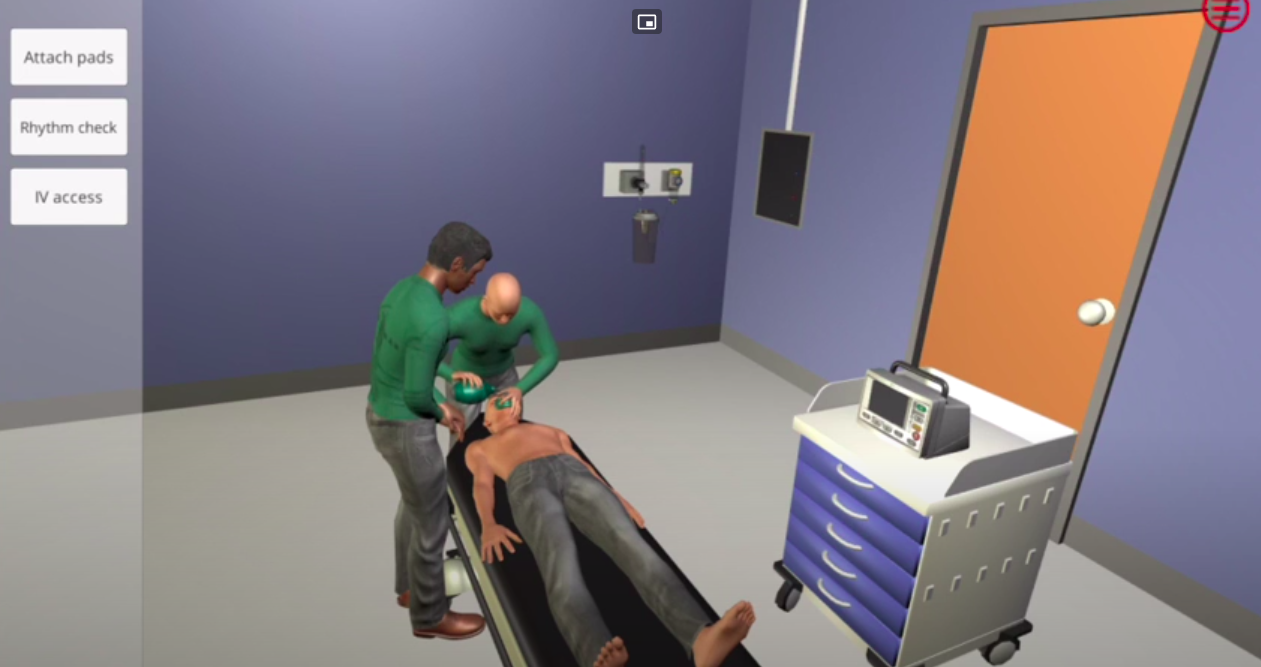
\includegraphics[width=\linewidth]{Virtu-ALS.png}
    \caption{Virtu-ALS}
    \label{fig:virtu-als}
\end{figure}

Virtu-ALS is a \emph{didactic} emergency care simulator mainly targeted at students and junior healthcare professionals, although its application as a reinforcement learning \emph{benchmark} was anticipated and accounted for by the authors \cite{virtu-als}.
Its most prominent feature is its visual nature (figure \ref{fig:virtu-als}): the user has access to a 3D-rendered virtual copy of a hospital room, view the monitor, press buttons on a defibrillator, etc.
However, the visual modality means that its observation space 
\begin{equation}
    \mathcal{O} \subset R^{307200}
\end{equation}

Such a high dimensionality of the observation space makes it an extremely challenging reinforcement learning task.
Tasks from this family have been solved with deep neural networks \cite{atari-rl}, however not only does it require a long and expensive training process, it also means that resulting treatment strategies are black box neural networks that no clinical expert understands.
This approach to decision making is extremely hard to introduce into clinical practice \cite{blackbox1,blackbox2}

Like most \emph{didactic} simulators, Virtu-ALS exhibits considerable \emph{confirmation bias} - any decision that's not supported by the standard emergency care protocol \cite{abcde,acls} is considered a mistake and rewarded negatively.

\section{Auto-ALS}

As our first model, we propose a low-dimensional version of \emph{Virtu-ALS}.
\emph{Auto-ALS} is a modification of Virtu-ALS that removes all the complexity of dealing with a visual 3D environment while retaining all the complexity of dealing with a patient that requires emergency care.
This is achieved by attaching an event listener to Virtu-ALS that registers all observable events that can occur in the simulator in response to the user's actions.
The events are listed in table \ref{tab:auto-als}, organized by which agent action can trigger which event.
\emph{Tick} is a special event that occurs every time the simulator is advanced a timestep, and is negatively reinforced, which when used with reinforcement learning algorithms discourages clinicaly unnecessary actions.

\texttt{MeasuredHeartRate, MeasuredRespRate, MeasuredCapillaryGlucose, MeasuredTemperature, MeasuredMAP, MeasuredSats, MeasuredResps} are \emph{measurements}, events that have a value $(\-infty; +\infty)$ associated with them.

\begin{table*}[]
\begin{tabular}{|p{0.4\linewidth}|p{0.45\linewidth}|c|}
\toprule
Agent actions &
  Patient reactions & Rewards
   \\
   \midrule
AssessResponse &
  ResponseVerbal,     ResponseGroan,     ResponseNone &
  \multirow{9}{*}{0} \\
AssessAirway &
  AirwayClear,     AirwayVomit,     AirwayBlood,     AirwayTongue &
   \\
AssessBreathing &
  BreathingNone,     BreathingSnoring,     BreathingSeeSaw,     BreathingEqualChestExpansion,     BreathingBibasalCrepitations,     BreathingWheeze,     BreathingCoarseCrepitationsAtBase,     BreathingPneumothoraxSymptoms,  VentilationResistance, \emph{MeasuredRespRate} &
   \\
AssessCirculation &
  RadialPulsePalpable,     RadialPulseNonPalpable, \emph{MeasuredHeartRate} &
   \\
AssessDisability &
  AVPU\_A,     AVPU\_U,     AVPU\_V, PupilsPinpoint,     PupilsNormal, \emph{MeasuredCapillaryGlucose} &
   \\
AssessExposure &
  ExposureRash,     ExposurePeripherallyShutdown,     ExposureStainedUnderwear, \emph{MeasuredTemperature} &
   \\
AssessDefibrillator &
   &
   \\
AssessMonitor &
  HeartRhythm0,     HeartRhythm1,     HeartRhythm2,     HeartRhythm3,     HeartRhythm4, \emph{MeasuredHeartRate}, \emph{MeasuredMAP}, \emph{MeasuredSats}, \emph{MeasuredResps} &
   \\
   DoNothing & & \\
   \midrule
ABG,     AirwayManoeuvres,     GiveAtropine,     GiveAdenosine,     GiveAdrenaline,     GiveAmiodarone,     GiveMidazolam,     Venflon,     Yankeur,     DrawBloods,     BPCuffOn,     BVM,     Guedel,     NRBMask,     DefibOn,     DefibAttachPads ,     DefibShock,     DefibCharge ,     DefibChangePaceCurrentDown,     DefibChangePaceCurrent,     DefibEnergyDown,     DefibEnergyUp,     DefibChangePaceRateDown,     DefibChangePaceRateUp,     DefibPace& 
   Blunder & $r_\text{blunder}$
   \\
   \midrule
   \multirow{2}{*}{Finish} & Failure & -1 \\
   & Success & 1 \\
   \midrule
   - & Tick & $r_\text{tick}$ \\
  \bottomrule
\end{tabular}
\caption{All actions and observations of Auto-ALS}
\label{tab:auto-als}
\end{table*}

    
The events in table \ref{tab:auto-als} only get registered if the agent has \emph{learnt} some piece of information, meaning that, for example, \verb|AirwayVomit| will only occur if the patient has vomit in their airway \emph{and} the agent checked the airway (which is part of the standard protocol \cite{abcde}).
Assessment skills (knowing where to look and how to establish the patient's state) are crucial for patient resuscitation, hence revealing all known health variables to the agent would jeopardize the simulation.


The observation vector in \emph{Auto-ALS} is based on all observations that have occurred between the beginning of the episode and current time.
However, more recent observations are more likely to still be relevant and should be given priority.
This is done with the following formula proposed in \cite{mpdp}:

\begin{equation}
     o^{+} = \langle o_1 \in O_1, \exp(t_1-t), \dots, o_n \in O_n, \exp(t_n-t), \rangle
\end{equation}

where $O_i$ is the value of the observation and $t$ is current time and $t_i$ is time when observation $i$ (for $i=5$, \verb|ResponseGroan|) has \emph{last} occurred and $\exp(t_i-t)$ represents its decaying relevance.
For \emph{measurements}, the $O_i$ equals the magnitude of the measurement, however, for binary obsevations $O_i$ would always be equal to one.
For memory efficiency, for all $i$ that correspond to binary observations, $O_i$ is skipped from the $o^{+} $ vector and the actual observation vector $o$ has size $36+7*2=50$, as opposed to $(36+7)*2=86$

See source code and documentation at \cite{auto-als}.